% Traceability: derived from supplement-b/examples/05_e10_recurrent_ring.tex
\subsection{Recurrent systems}

\subsubsection{Recurrent ring witness}
\label{man:recurrent-ring-witness}
\colabbadge{manual/notebooks/04e_recurrent_ring.ipynb}

A cited recurrent-ring row is fixed first and then displayed as a compact recurrent-system witness.

\begin{table}[H]
\centering
\caption{Recurrent ring witness row.}
\label{tab:recurrent-ring-witness-row}
\begin{threeparttable}
\small
\pgfplotstabletypeset[
  columns={row_id,topology,Rloss_trit_per_bip,B_star_mode_bip,Lambda_hat_ticks,Rloss_biz_derived},
  columns/row_id/.style={column name=Row,string type,column type=l},
  columns/topology/.style={column name=Topology,string type,column type=l},
  columns/Rloss_trit_per_bip/.style={column name={$R_{\mathrm{loss}}$ [trit/bip]},fixed,precision=6},
  columns/B_star_mode_bip/.style={column name={$B^*$ [bip]},fixed,precision=0},
  columns/Lambda_hat_ticks/.style={column name={$\widehat\Lambda$ [ticks]},fixed,precision=0},
  columns/Rloss_biz_derived/.style={column name={$R^{(\mathrm{biz})}_{\mathrm{loss}}$ [biz]},fixed,precision=6}
]{data/temporal/01_recurrent_ring_summary.csv}
\ManualTableNote{This compact display reuses the cited recurrent-ring ledger as a recurrent-system witness across scales.}
\end{threeparttable}
\end{table}

\begin{figure}[H]
\centering
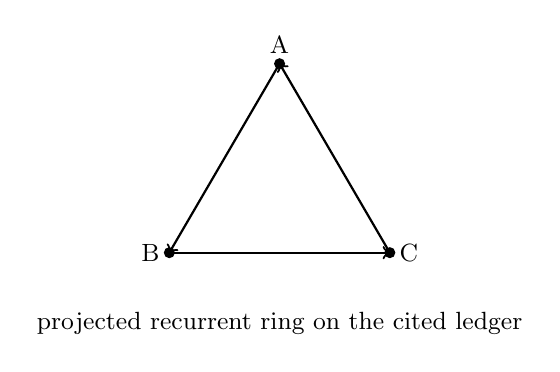
\begin{tikzpicture}[x=1cm,y=1cm, every node/.style={font=\small}]
  \coordinate (A) at (0,1.6);
  \coordinate (B) at (-1.4,-0.8);
  \coordinate (C) at (1.4,-0.8);
  \draw[thick,->] (A) -- (B);
  \draw[thick,->] (B) -- (C);
  \draw[thick,->] (C) -- (A);
  \fill (A) circle (2pt) node[above] {A};
  \fill (B) circle (2pt) node[left] {B};
  \fill (C) circle (2pt) node[right] {C};
  \node at (0,-1.7) {projected recurrent ring on the cited ledger};
\end{tikzpicture}
\caption{Recurrent ring witness.}
\label{fig:recurrent-ring-witness}
\end{figure}

The cited recurrent ledger carries the CK-mismatch and cut-residual diagnostics used to distinguish recurrent projection effects from kernel bias.
